\documentclass{article}
\usepackage{amsmath}
\usepackage{graphicx}

\title{Dirichlet Kernel Visualization}
\author{Your Name}

\begin{document}

\maketitle

\section{Introduction}

This document describes the usage and visualization of the Dirichlet kernel function, implemented in the Jupyter Notebook \texttt{dirichlet.ipynb}.

\section{Dirichlet Kernel Function}

The Dirichlet kernel function is defined as:

\[
D_n(x) = \frac{\sin((n + 0.5)x)}{\sin(0.5x)}
\]

In the notebook, this function is implemented as follows:

\begin{verbatim}
import numpy as np
import matplotlib.pyplot as plt

def dirichlet_kernel(x, n):
    return np.sin((n + 0.5) * x) / np.sin(0.5 * x)
\end{verbatim}

\section{Usage}

To visualize the Dirichlet kernel function, follow these steps:

\begin{enumerate}
    \item Clone the repository:
    \begin{verbatim}
    git clone https://github.com/your-repo/dirichlet-visualization.git
    cd dirichlet-visualization
    \end{verbatim}

    \item Ensure you have the necessary Python packages installed:
    \begin{verbatim}
    pip install numpy matplotlib jupyter
    \end{verbatim}

    \item Open the Jupyter Notebook:
    \begin{verbatim}
    jupyter notebook dirichlet.ipynb
    \end{verbatim}

    \item Run the notebook cells to generate the Dirichlet kernel plots.
\end{enumerate}

\section{Example Plot}

Below is an example plot generated by the notebook:

\begin{figure}[h]
    \centering
    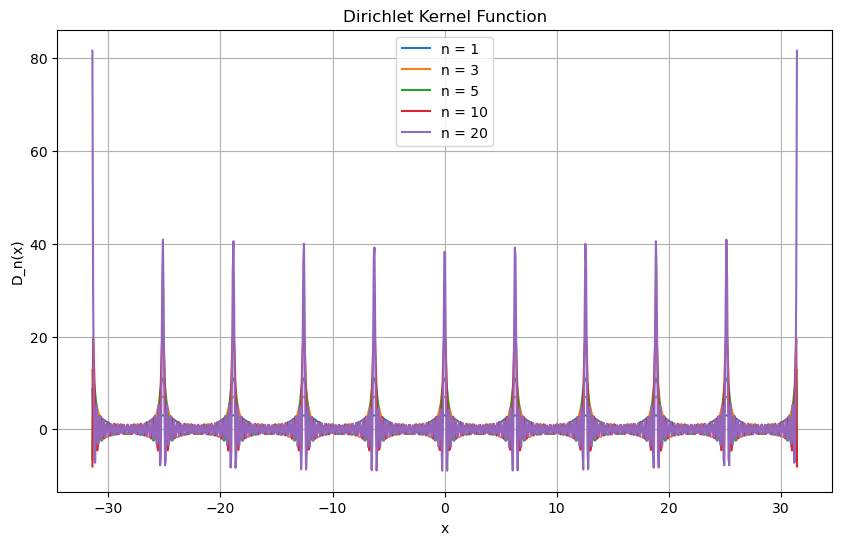
\includegraphics[width=\textwidth]{images/dirichlet_kernel_plot.png}
    \caption{Dirichlet Kernel Function Plot}
\end{figure}

\section{Notes}

\begin{itemize}
    \item The \texttt{dirichlet\_kernel} function computes the Dirichlet kernel for given values of \texttt{x} and \texttt{n}.
    \item Multiple values of \texttt{n} can be visualized on the same plot to compare the behavior of the Dirichlet kernel.
\end{itemize}

\end{document}
